\scanpage{7}
\mspage{5}
\margin{\figure{\begin{tikzpicture}\draw (0,0) .. controls (.1,-.2) and (.4,-.5) .. (.6,-.7);\end{tikzpicture}}}

\uline{pg60}\quad Je n'ai ps confiance en ``il est immédiat'' de 6.4.
\margin{\figure{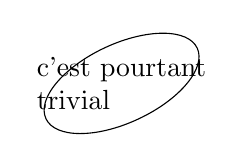
\begin{tikzpicture}[baseline=(t.base)]\node[align=left] (t) {c'est pourtant\\trivial};\draw[rotate=25] (0,0) ellipse (1.06 and 0.50);\end{tikzpicture}}}

\uline{pg61, 61 bis} : Je n'ai pas lu.

Il me semble qu'il doit être possible de définir, à isogénie près, des ``parties finies'' et ``parties toriques'', ayant le bon rang --
\margin{\figure{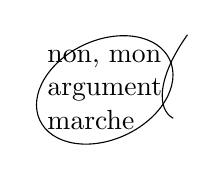
\begin{tikzpicture}[baseline=(t.base)]\node[align=left] (t) {non, mon\\argument\\marche};\draw[rotate=25] (0,0) ellipse (0.91 and 0.63);\draw (1.05,0.70) .. controls (0.66,0.15) and (0.66,-0.25) .. (0.87,-0.36);\end{tikzpicture}}}

\uline{pg\unsure{64|67}/\unsure{bis}} : \deleted{\unsure{voir}} (réf. à Serre pour \unsure{l'indép.|l'insép.} de $\ell$ ligne 11 ?)

Un peu malhonnête d'être si bref, car 6.6 est utilisé en 5.13.
\margin{\figure{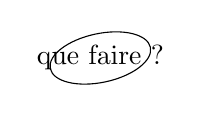
\begin{tikzpicture}[baseline=(t.base)]\node (t) {que faire ?};\draw[rotate=12] (0,0) ellipse (0.65 and 0.31);\end{tikzpicture}}}

\figure{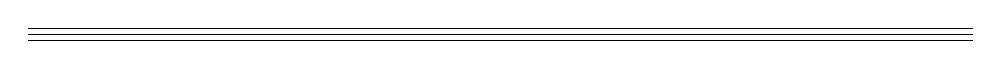
\begin{tikzpicture}\draw (0,0)--(12,0);\draw (0,-0.08)--(12,-0.08);\draw (0,-0.16)--(12,-0.16);\end{tikzpicture}}

\figure{
\begin{tikzpicture}[baseline=(t.base)]\node (t) {7};\draw (0,0) ellipse (0.27 and 0.25);\end{tikzpicture}}
\uline{p65}.\quad $A_0$ n'est pas défini\margin{si}

\uline{p.67}\quad (7.1.4)\quad français --
\margin{\figure{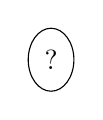
\begin{tikzpicture}[baseline=(t.base)]\node (t) {?};\draw (0,0) ellipse (0.29 and 0.40);\end{tikzpicture}}}

\figure{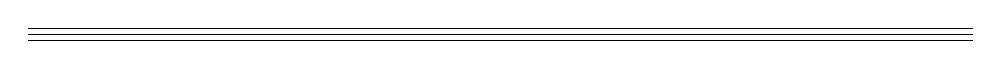
\begin{tikzpicture}\draw (0,0)--(12,0);\draw (0,-0.08)--(12,-0.08);\draw (0,-0.16)--(12,-0.16);\end{tikzpicture}}

\figure{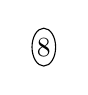
\begin{tikzpicture}[baseline=(t.base)]\node (t) {8};\draw (0,0) ellipse (0.15 and 0.24);\end{tikzpicture}}

\figure{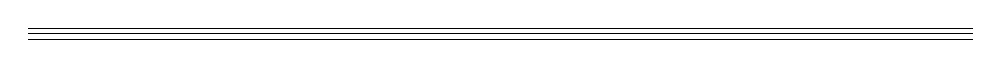
\begin{tikzpicture}\draw (0,0)--(12,0);\draw (0,-0.07)--(12,-0.07);\draw (0,-0.14)--(12,-0.14);\end{tikzpicture}}

\figure{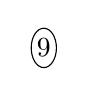
\begin{tikzpicture}[baseline=(t.base)]\node (t) {9};\draw (0,0) ellipse (0.16 and 0.25);\end{tikzpicture}}
\uline{p80}\quad 9.2.3\quad $u$ plutôt que $u(\unsure{g|q})$

\uline{p82}\quad (9.3.3)\quad $+$ compatibilité avec $R$ ? --

\uline{p87}\quad 9.4.\quad $S$ \uuline{strictement} hensélien ? (on le suppose en p88, $\ell-9$)

pas d'hyp. d'excellence ?

\uline{p91} : 9.5.8.\quad Ne mettrais-tu pas une génuflexion ``\unsure{au|en} signe près''.

\uline{pg92 bis}\quad $S$ est-il strictement hensélien ?

\figure{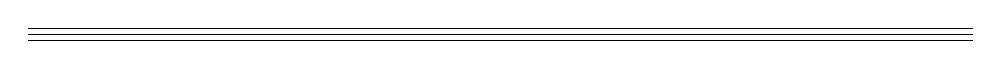
\begin{tikzpicture}\draw (0,0)--(12,0);\draw (0,-0.08)--(12,-0.08);\draw (0,-0.16)--(12,-0.16);\end{tikzpicture}}

\figure{
\begin{tikzpicture}[baseline=(t.base)]\node (t) {10};\draw (0,0) ellipse (0.26 and 0.25);\end{tikzpicture}}
\uline{pg98}\quad 10.5.3.\quad Une extension de $K$ (qui ici est infini) est-elle requise ??

10.5.4.\quad Dire \uline{où} on fera ces vérifications --

\margin{6}
